\chapter{Grundlagen Nanoprobing}
In diesem Kapitel werden die Grundlagen des Nanoprobing behandelt. Geräte und Software, die zum Einsatz kommen, werden erklärt.

Die Firma Kleindiek Nanotechnik stellt Geräte und Messelektronik für das Nanoprobing her und ist auf diesem Gebiet weltweit führend \cite{kn}.
Für eine ausführliche Erklärung von Nanoprobing sowie einen Einblick in die Firma Kleindiek Nanotechnik GmbH, wird auf das Video von Roman Hartung verwiesen. \cite{youtube-derbauer} 

\section{Nanoprobing}
Nanoprobing ist eine Technik aus dem Bereich der Nanoelektronik, die zur Analyse von Bauteilen im Nanometerbereich eingesetzt wird. Die Technik verwendet spezielle Messspitzen, um mit nanoskaligen Strukturen zu interagieren und deren Eigenschaften zu bestimmen. Ein wichtiges Anwendungsgebiet in der Halbleiterindustrie ist die Fehleranalyse von Transistoren. Dabei werden elektrische Fehler wie Kurzschlüsse, Unterbrechungen, Widerstände und Leckpfade detektiert und analysiert.

\subsection{Prober Shuttle}
\begin{figure}[htbp]
\centerline{
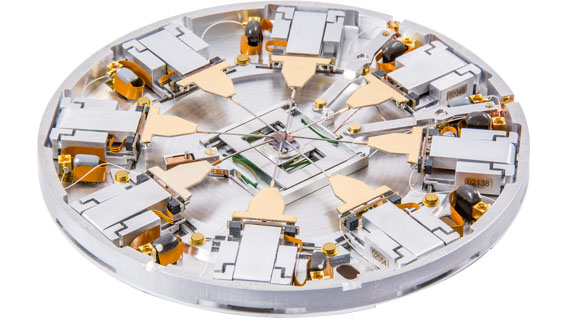
\includegraphics[width=.7\textwidth, angle=0]{img/ps8.jpg}}
\caption{Ein voll bestücktes Prober Shuttle (PS8)}
\label{fig:PS8}
\begin{small}
\end{small}
\end{figure}
Die Firma Kleindiek Nanotechnik hat das Prober Shuttle entwickelt, ein System, das je nach Modell (PS4 oder PS8) mit vier bis acht Manipulatoren ausgestattet ist. Jeder Manipulator kann in drei Achsen bewegt werden: A für links/rechts, B für oben/unten, C für rein/raus. Durch den Einsatz eines speziell entwickelten Piezomotors arbeiten die Manipulatoren im Subnanometerbereich und sind damit in der Lage, die Kontakte der neuesten Transistorgeneration in der Chipfertigung präzise anzufahren und diese auf Fehler zu überprüfen.

Das PS8e ist eine spezielle Version des Prober Shuttles. Das „e“ steht für „encoded“ und bezieht sich auf kapazitive Felder unter den Manipulatoren, die deren Position bestimmen können. Nach einmaliger Kalibrierung kann das Prober Shuttle die Messspitzen bis auf \SI{10}{\micro\metre} zusammenfahren. Aufgrund der geringen Größe der Kontakte – einige zehn Nanometer – ist jedoch eine manuelle Steuerung der Manipulatoren für die Kontaktierung erforderlich.

Die Ansteuerung der Manipulatoren erfolgt über das Nanocontrol (NC). Es bietet Drehknöpfe zur Ansteuerung, verarbeitet aber auch über RS232 gesendete Befehle und steuert den Manipulator entsprechend an. Jeder Manipulator hat ein eigenes NC, diese sind zusammen mit der Messelektronik in einem Rack montiert. Ein voll bestücktes Rack ist in Abbildung \ref{fig:workplace} zu sehen.

\subsection{Messspitzen}
Die Messspitzen aus massivem Wolfram sind in verschiedenen Ausführungen erhältlich. Der Schaftdurchmesser beträgt \SI{0,25}{\milli\metre}, der Spitzenradius variiert zwischen \SI{250}{\nano\metre} und \SI{5}{\nano\metre}. Aufgrund der unterschiedlichen Spitzenradien können die Spitzen in den Mikroskopiebildern zum Teil sehr unterschiedlich aussehen. Wie in Abbildung \ref{subfig:MesoscopeTips2} zu erkennen ist.
\begin{figure}[h]
\centerline{
\subfigure[Messspitzen]{
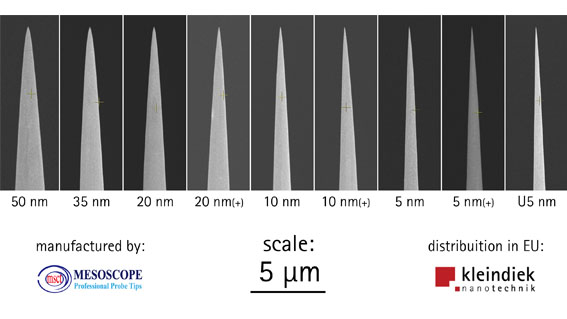
\includegraphics[width=.5\textwidth, angle=0]{img/mesoscope_tips.png}
\label{subfig:MesoscopeTips1}}\hfill
\subfigure[Auf Kontakten abgesetzte Messspitzen]{
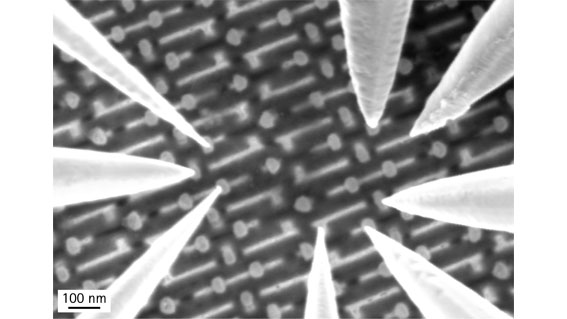
\includegraphics[width=.5\textwidth, angle=0]{img/mesoscope_tips_probing.png}
\label{subfig:MesoscopeTips2}}}
\caption{Messspitzen der Firma Mesoscope in verschiedenen Ausführungen. Nach Spitzenradii sortiert \ref{subfig:MesoscopeTips1} und abgesetzt auf den Kontakten mehrerer Transistoren \ref{subfig:MesoscopeTips2}}
\label{fig:MesoscopeTips}
\begin{small}
\end{small}
\end{figure}
\newpage
\section{Rasterelektronenmikroskop}
Das Rasterelektronenmikroskop (REM) ist in der Halbleiterindustrie unverzichtbar, da es die Oberflächentopografie und -zusammensetzung von Proben mit einer Auflösung bis zu \SI{10}{\nano\metre} sichtbar machen kann.
Im Gegensatz zu herkömmlichen Lichtmikroskopen arbeitet das REM mit einem fokussierten Elektronenstrahl, der beim Auftreffen auf die Probenoberfläche eine Reihe von Signalen erzeugt. Diese Signale werden dann in ein sichtbares Bild umgewandelt. Zwei Arten von Elektronen-Proben-Wechselwirkungen können unterschieden werden: elastische und inelastische Wechselwirkungen. Elastische Wechselwirkungen führen zur Erzeugung von Rückstreuelektronen (BSE), während inelastische Wechselwirkungen zur Erzeugung von Sekundärelektronen (SE) führen. Diese werden zusammen mit anderen Signalen wie Röntgenstrahlung und Augerelektronen zur Bildanalyse und -erzeugung verwendet.

\begin{wrapfigure}{r}{0.5\linewidth}
    \centering
    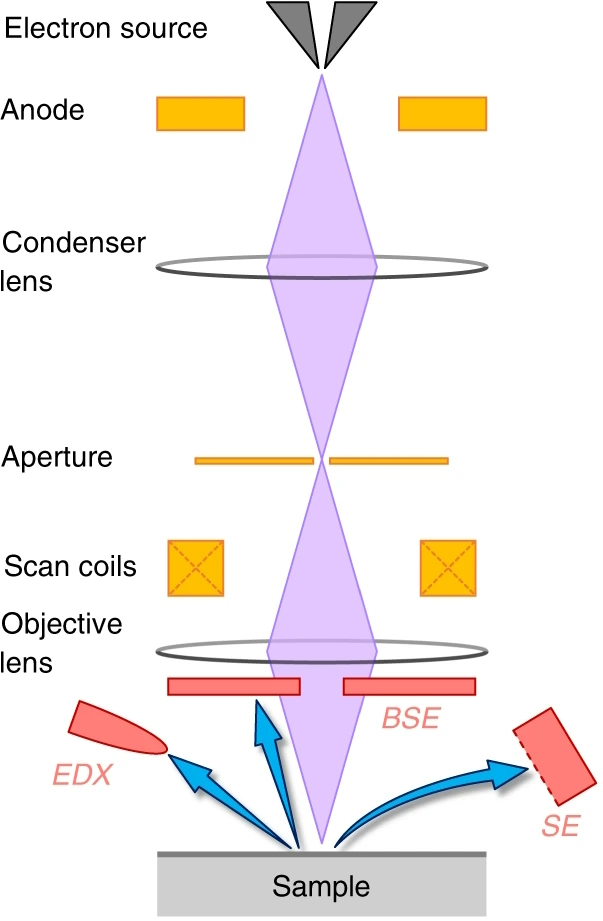
\includegraphics[width=\linewidth]{img/SEM.jpg}
    \caption{Grundlegender Aufbau eines Rasterelektronenmikroskops. Quelle: nature.com \cite{Shah.2019}}
    \label{fig:sem}
\end{wrapfigure}
Die Arbeitsweise eines REM besteht aus mehreren Schritten. Dargestellt sind diese in Abbildung \ref{fig:sem}. Zunächst erzeugt eine Elektronenkanone einen stabilen Elektronenstrahl, der auf einen kleinen Punkt gerichtet ist. Es gibt verschiedene Arten von Elektronenkanonen, zum Beispiel Wolfram-Elektronenkanonen, Lanthanhexaborid (LaB6)-Elektronenkanonen und Feldemissionskanonen. Der erzeugte Elektronenstrahl wird durch Linsen – Kondensorlinsen und Objektivlinsen – gebündelt und auf die Probe fokussiert. Die Kondensorlinsen richten den Elektronenstrahl parallel aus, während die Objektivlinsen den Strahl auf einen Punkt fokussieren. Zur Bildentstehung lenkt eine Abtastspule den Strahl entlang der x- und y-Achse ab, um die gesamte Probe abzudecken. Dies ermöglicht eine stufenlose Vergrößerung von 10x bis 2.000.000x. Der Sekundärelektronendetektor schließlich detektiert die emittierten Sekundärelektronen, die eine feine topografische Information liefern.

Die Eindringtiefe des Elektronenstrahls und die Oberflächenauflösung hängen von der Energie des Elektronenstrahls und der Zusammensetzung der Probe ab. Hier gilt es, ein Gleichgewicht zu finden und je nach Anforderung die optimale Strahlenergie zu bestimmen \cite{INKSON201617}\cite{Zhou2007}.

\begin{figure}[h]
    \centering
    \subfigure[\SI{500}{\volt}]{\label{subfig:lowvoltage1}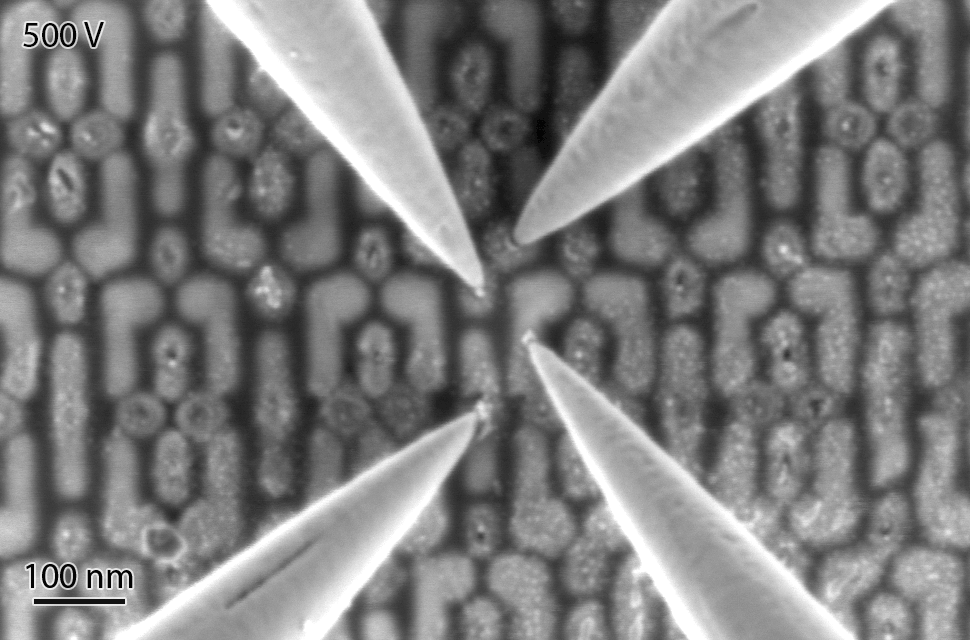
\includegraphics[width=.45\textwidth, angle=0]{img/7-nm-low-voltage_anim_page_0001.png}}
    \subfigure[\SI{300}{\volt}]{\label{subfig:lowvoltage2}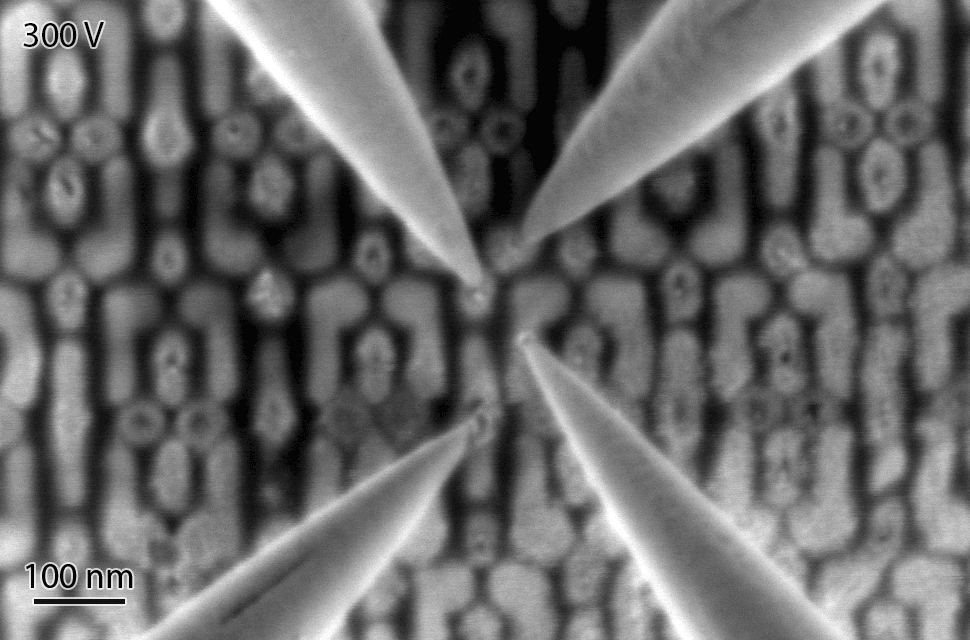
\includegraphics[width=.45\textwidth, angle=0]{img/7-nm-low-voltage_anim_page_0002.png}}\\
    \subfigure[\SI{200}{\volt}]{\label{subfig:lowvoltage3}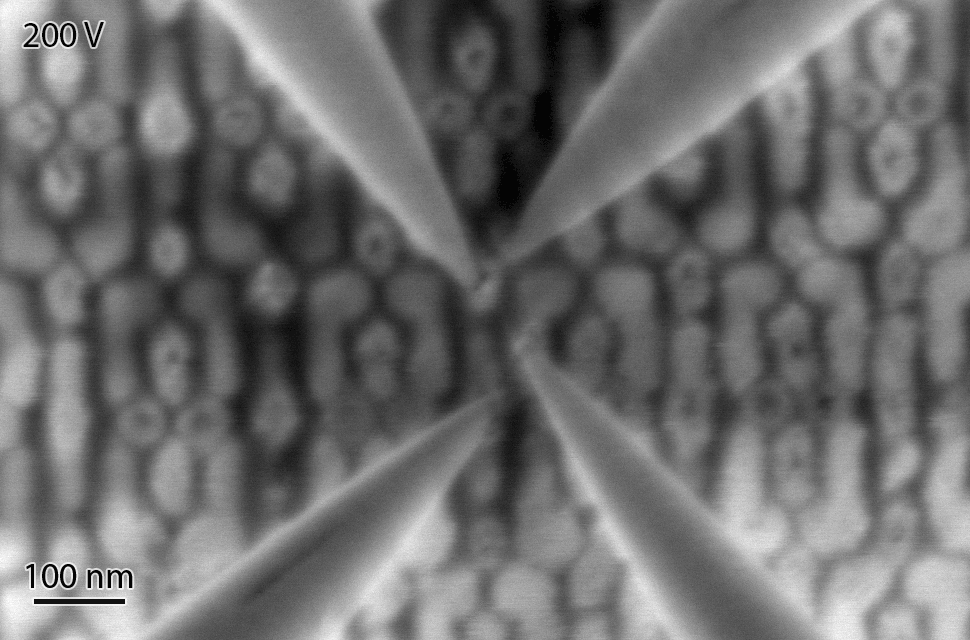
\includegraphics[width=.45\textwidth, angle=0]{img/7-nm-low-voltage_anim_page_0003.png}}
    \subfigure[\SI{150}{\volt}]{\label{subfig:lowvoltage4}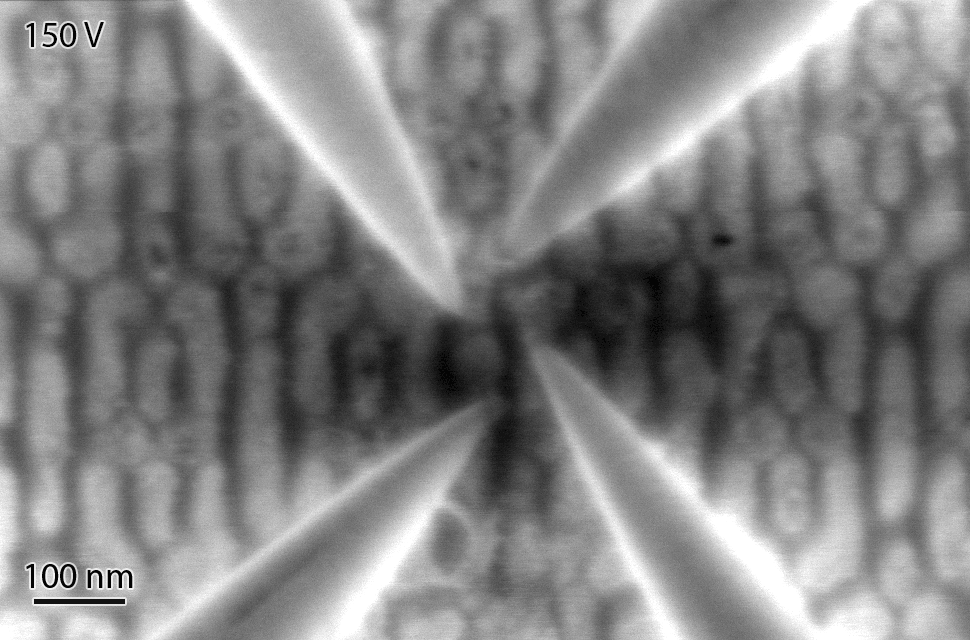
\includegraphics[width=.45\textwidth, angle=0]{img/7-nm-low-voltage_anim_page_0004.png}}
    \captionsource{Visualisierung der Messspitzen bei verschiedenen Beschleunigungsspannungen.}{Kleindiek Nanotechnik GmbH}
    \label{fig:lowvoltages}
\end{figure}
\newpage
Bei der Untersuchung von Transistoren mit einem REM spielt die Beschleunigungsspannung, mit der die Elektronen auf die Probe geschossen werden, eine besonders wichtige Rolle. Ist die Beschleunigungsspannung zu hoch, kann die empfindliche Struktur der Transistoren beschädigt werden. Für die Analyse neuester Chiptechnologien wird daher eine Beschleunigungsspannung von weniger als 200 Volt benötigt. Wie die Abbildung \ref{fig:lowvoltages} zeigt, wirkt sich diese niedrige Beschleunigungsspannung jedoch negativ auf die Bildqualität aus, da sie eine Vielzahl von Bildstörungen verursacht. Dies äußert sich unter anderem in einer geringeren Bildschärfe und einem geringeren Kontrast.
\subsection*{ZEISS GeminiSEM Mikroskop und ZEISS SmartSEM Software}
Das in dieser Arbeit verwendete REM ist ein ZEISS GeminiSEM 300, es erfüllt die höchsten Anforderungen an Subnanometer-Imaging, Analytik und Probenflexibilität \cite{geminisem}.
Gesteuert wird es über die \glqq ZEISS SmartSEM Software\grqq{}, die eine benutzerfreundliche Oberfläche zur effizienten Steuerung und Optimierung des REM-Betriebs bietet.
Mit der \glqq SmartSEM Remote API\grqq{} stellt ZEISS Entwicklern eine Schnittstelle zur Fernsteuerung des Mikroskops zur Verfügung.
So können über speziell entwickelte Skripte analoge und digitale Parameter gesetzt, der Status des Mikroskops ausgelesen und Befehle gesendet werden.
\newpage
\section{Kleindiek Nanotechnik: Arbeitsplatz}
\begin{figure}[h]
    \centering
    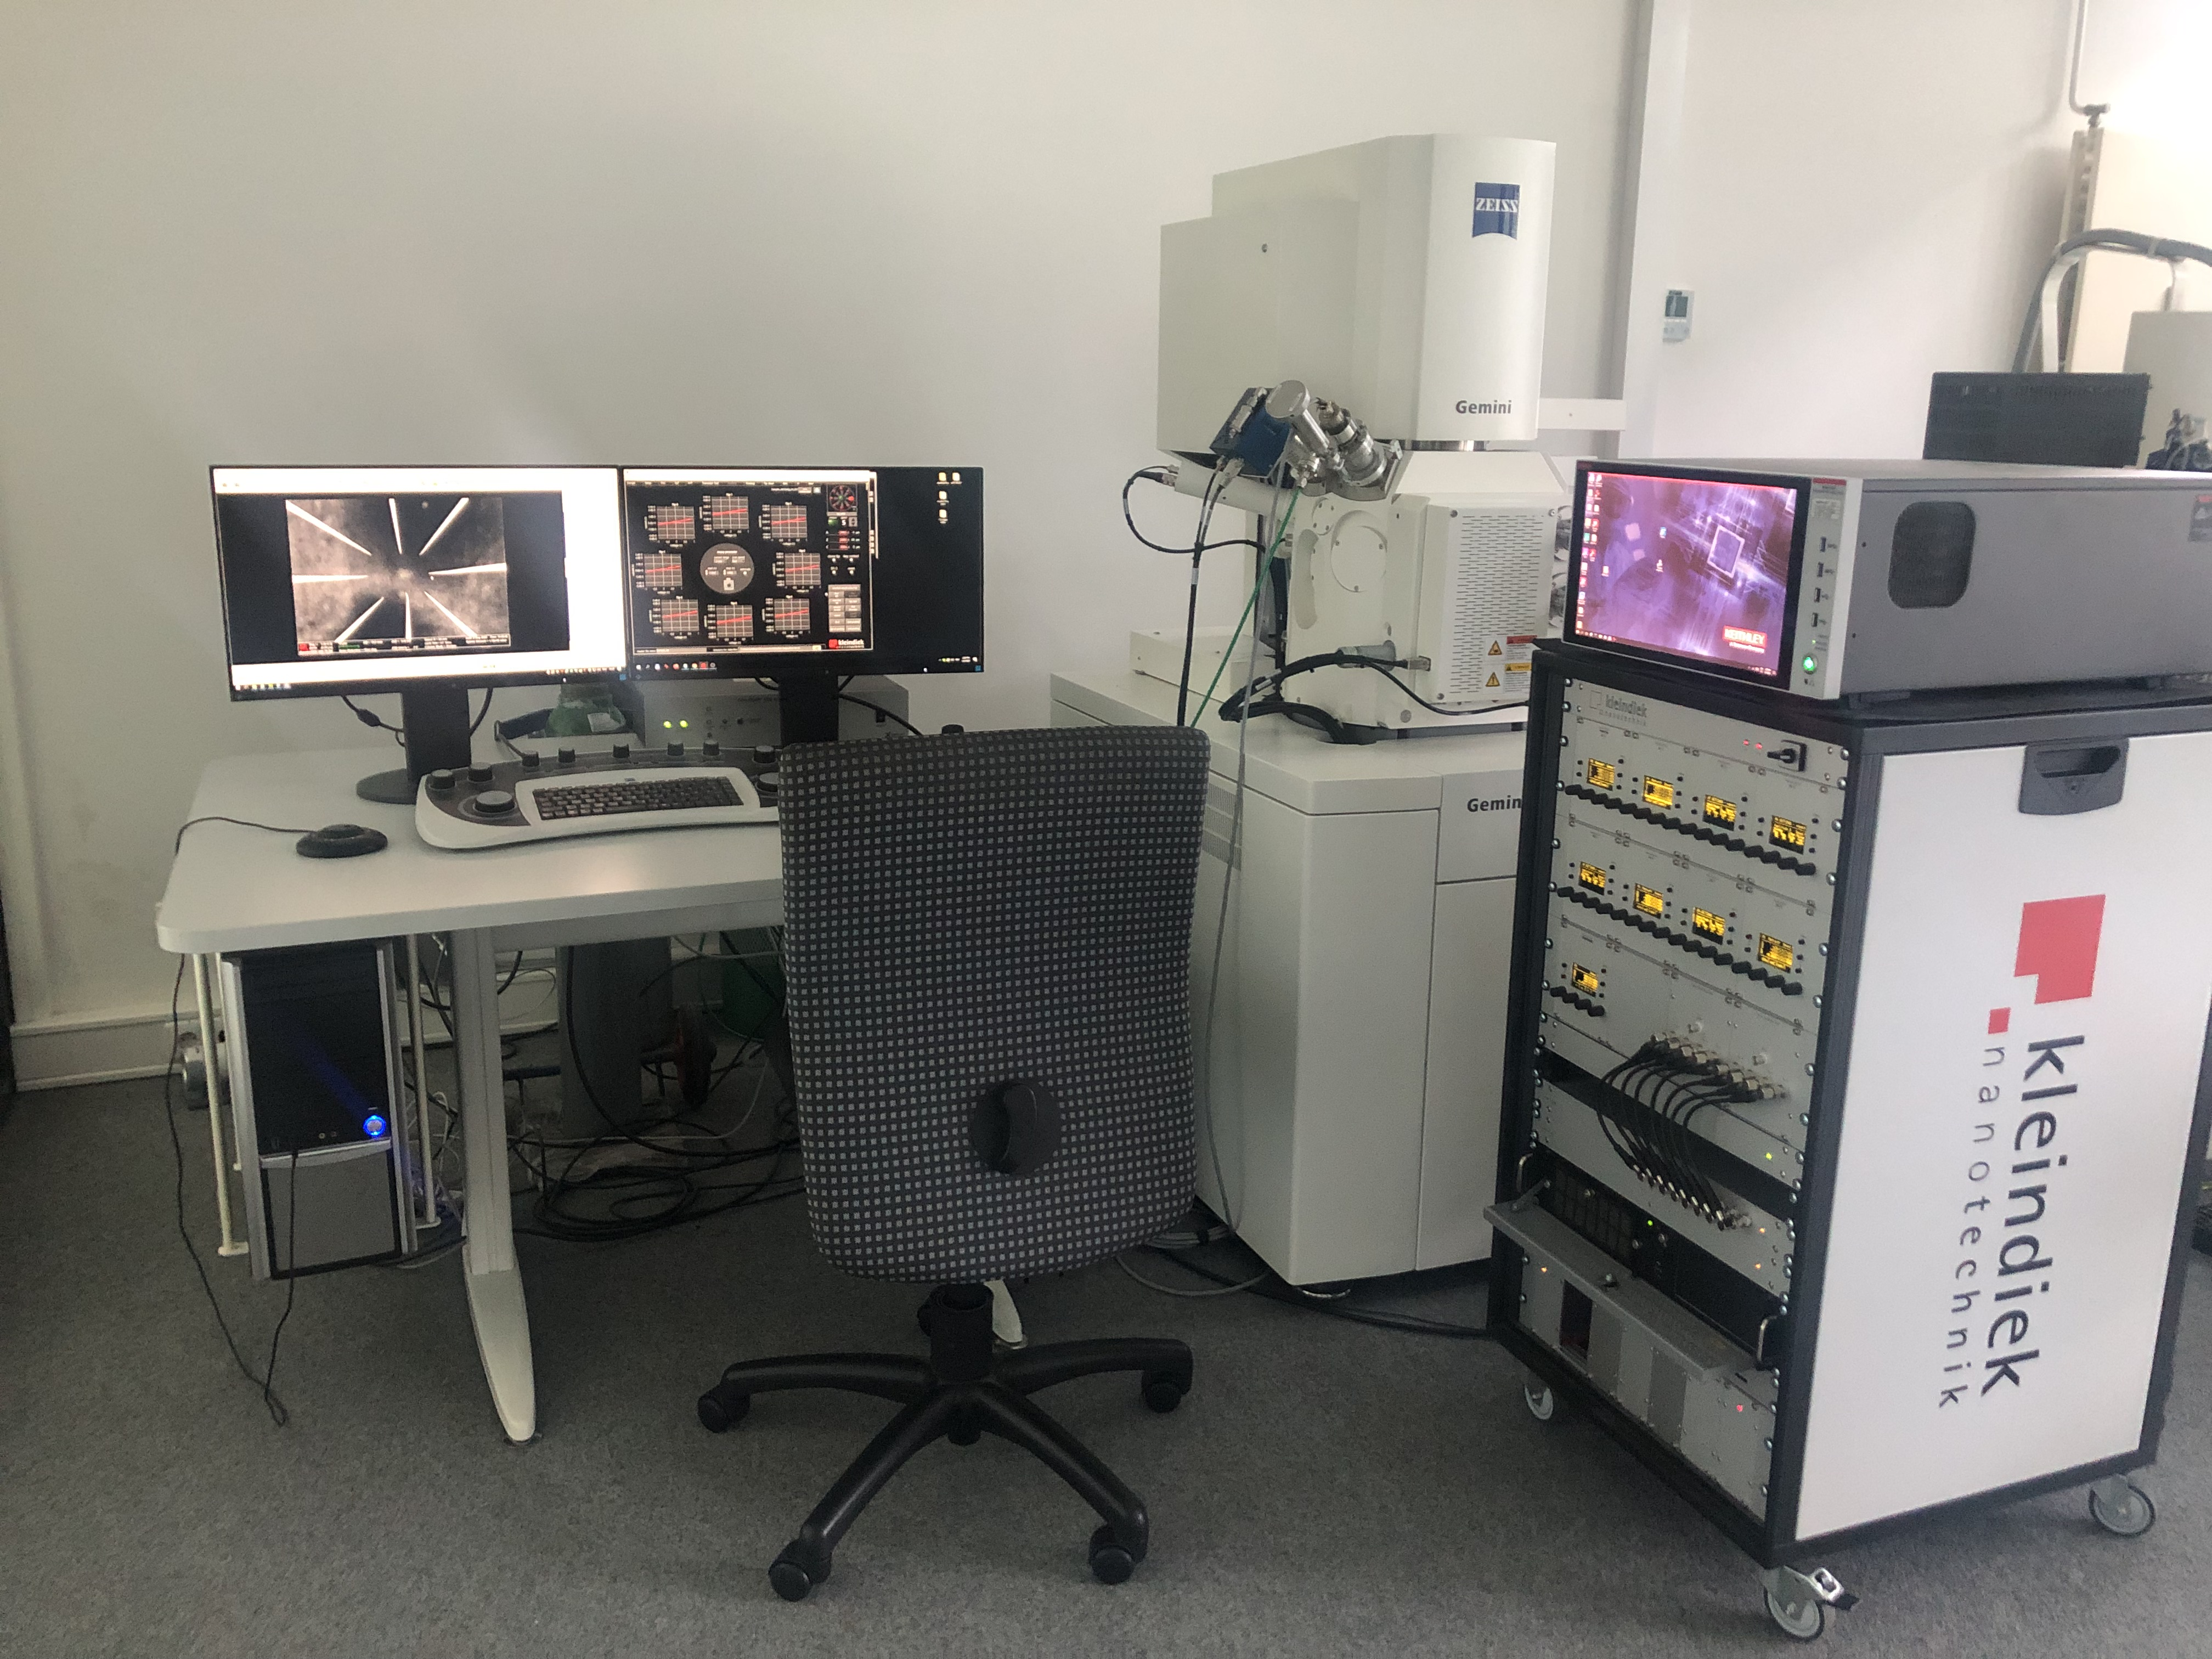
\includegraphics[width=\linewidth]{img/workplace.JPG}
    \captionsource{Arbeitsplatz bei Kleindiek.}{Kleindiek Nanotechnik GmbH}
    \label{fig:workplace}
\end{figure}
Der verwendete Arbeitsplatz ist in Abbildung \ref{fig:workplace} dargestellt.
Er ist mit einem GeminiSEM 300 ausgestattet, in das ein voll ausgestattetes PS8e eingebaut ist. Das Mikroskop wird über den links zu sehenden PC gesteuert.
Das Rack (rechts neben dem Mikroskop) enthält neun Nanocontroller. Acht für die Steuerung der Manipulatoren und einer für die Stage, auf der die Probe montiert ist. Die gesamte Messelektronik und ein weiterer PC sind ebenfalls im Rack untergebracht. Alle Geräte werden über die von ZEISS und Kleindiek zur Verfügung gestellte Software ferngesteuert.

Da im Rahmen dieser Arbeit eine eigens entwickelte Steuerung zum Einsatz kommt, werden die Nanocontrols und das REM über einen eigenen Laptop gesteuert und nicht über die PCs am Arbeitsplatz und im Rack.